\documentclass[10pt,letterpaper]{article}
\usepackage[top=0.85in,left=2.75in,footskip=0.75in]{geometry}
\usepackage{amsmath,amssymb}
\usepackage{changepage}
\usepackage[utf8]{inputenc}
\usepackage{textcomp,marvosym}
\usepackage{cite}
\usepackage{nameref}
\usepackage[pdftex,
            pdfauthor={Peter Reintjes},
            pdftitle={EvoStat Level Monitoring System},
            pdfsubject={Level Monitoring},
            pdfkeywords={OpenCV Python},
            pdfproducer={Latex with hyperref},
            pdfcreator={pdflatex}]{hyperref}

\hypersetup{
    colorlinks=true,
    linkcolor=blue,
    filecolor=magenta,      
    urlcolor=cyan,
}
\usepackage[right]{lineno}
\usepackage{microtype}
\DisableLigatures[f]{encoding = *, family = * }
\usepackage[table]{xcolor}
\usepackage{array}
\usepackage{listings}
\newcolumntype{+}{!{\vrule width 2pt}}
\newlength\savedwidth
\newcommand\thickcline[1]{%
  \noalign{\global\savedwidth\arrayrulewidth\global\arrayrulewidth 2pt}%
  \cline{#1}%
  \noalign{\vskip\arrayrulewidth}%
  \noalign{\global\arrayrulewidth\savedwidth}%
}

% \thickhline command for thick horizontal lines that span the table
\newcommand\thickhline{\noalign{\global\savedwidth\arrayrulewidth\global\arrayrulewidth 2pt}%
\hline
\noalign{\global\arrayrulewidth\savedwidth}}

\usepackage{enumitem}
\setlist{nosep}
\raggedright
\setlength{\parindent}{0.5cm}
\textwidth 5.25in 
\textheight 8.75in

\usepackage[aboveskip=1pt,labelfont=bf,labelsep=period,justification=raggedright,singlelinecheck=off]{caption}
\renewcommand{\figurename}{Fig}

% Remove brackets from numbering in List of References
\makeatletter
\renewcommand{\@biblabel}[1]{\quad#1.}
\makeatother

% Leave date blank
\date{}
% Header and Footer with logo
\usepackage{lastpage,fancyhdr,graphicx,wrapfig}
\usepackage{epstopdf}
\pagestyle{myheadings}
\pagestyle{fancy}
\fancyhf{}
\setlength{\headheight}{27.023pt}
%\lhead{
\includegraphics[width=2.0in]{PLOS-submission.eps}}
%\rfoot{\thepage/\pageref{lastpage}}
\renewcommand{\footrule}{\hrule height 2pt \vspace{2mm}}
\fancyheadoffset[L]{2.25in}
\fancyfootoffset[L]{2.25in}
% customize
\lfoot{\sf Innatrix Internal Document}

\begin{document}

\title{EvoStat Level Monitoring System}
\author{Peter Reintjes}
\date{\today}
\maketitle

\vspace*{0.2in}
\begin{flushleft}
\includegraphics[scale=0.5]{{phagestat}.jpg}
\end{flushleft}

{\it The EvoStat liquid-level control system consists of two distict parts: Monitoring and Control, which are accomplished by separate programs.  This report focuses on the monitoring program (alevel.py), a Python/OpenCV\cite{opencv} program which observes and reports the levels of vessels within the main EvoStat chamber.  The main EvoStat control program requires this level information to maintain volumes, cell density, and flow rates in the various chambers to support experiments in the continuous evolution of bacteriophage\cite{pace}.}

\section*{Introduction}

The {\bf alevel.py} program is a Python program which takes an image from a digital camera and determines the individual liquid levels in transparent containers within the image.  The EvoStat system uses the program to report the liquid levels of up to five vessels, one 2-liter host-cell cultivator and four 250mL lagoons.

\section*{Level Detection in the EvoStat}
Whenever a level reading is to be taken, {\bf alevel.py} reads a text file {\bf .previous} which specifies for each vessel:

\begin{enumerate}[itemsep=1pt, topsep=2pt, partopsep=0pt]
\item Area of the image in which the meniscus appears
\item Recommended intensity amplification (images to sum)
\item Recommended contrast (gain and threshold) settings
\end{enumerate}
Here is an example of the {\bf .previous} file containing the recommended settings and vessel locations.  The {\bf reticule} entry refers to the red reference LEDs used for level calibration.  The absence of a bounding box indicates that the reticules can be anywhere within the image area.
\begin{verbatim}
# (Vessel,oldPt,BBox,Contrast-iter, Contrast-mul, Contrast-off,')
#               Erode-iter, Dilate-iter, Amplify-iter, Amp-factor')
# (name, (x,y), ((uy,lx),(ly,rx)), 1, 1.2, -80, 2, 2, 3, 0.7)')
# lagoon   1, 1.5972, -90, 2, 2, 3, 0.7)]
[('reticule', 0, 1.4, -80, 180, 1, 4, 3, 0.4),
 ('host0', (47, 22), ((40, 120), (214, 380)), 1, 1.2, -80, 2, 2, 2, 0.4),
 ('lagoon1', (84, 71), ((340, 50), (460, 260)), 1, 1.1, -110, 2, 2, 3, 0.7)]
\end{verbatim}

The file is named {\bf .previous} because the program will try these recommended values for contrast and intensity settings but vary them until it can get a good level reading.  If the user specified the {\bf update} option when invoking {\bf alevel.py} a new file will be written with the contrast and intensity values actually used.  The next time the program is run, these settings may be able to get a good level reading without the need to vary them.  The program may also adjust the bounding boxes to be smaller and centered on the meniscus that was actually measured.

\subsection*{Camera Settings}
The unusual (low) light conditions inside the EvoStat may require a camera to be initialized with specific exposure, contrast, and saturation settings. While many cameras have automatic exposure modes, detection can often be improved with custom settings to match the dark conditions and our use of primary colors: red for the reticules, green for the liquid menisci.

One of the legacies of
Windows\textsuperscript{\textregistered}
and other closed systems is that each camera manufacturer has to produce a program for the (closed) operating system for each of their cameras.  Linux systems have kept up pretty well with a tool called guvcview which knows about many cameras -- especially the cheap ones.  This interactive program can be used to modify settings on many cameras and save those settings in a file with the {\bf .gpfl} suffix.  This file can be used to initialize the camera when the program starts by calling the program {\bf uvcdynctrl}.

After making the necessary image adjustments to the camera at {\bf /dev/video0} with {\bf guvcview} and saving the settings in the file {\bf evostat.gpfl}, the level monitor program (or any other process) can run the following command to restore the camera to these settings:
\begin{verbatim}
       /usr/bin/uvcdynctrl -L evostat.gpfl --device=/dev/video0
\end{verbatim}

Although the EvoStat programs are otherwise portable between Linux and
Windows\textsuperscript{\textregistered}
systems, we know of no comparable program that would make this method
of camera initialization available on
Windows\textsuperscript{\textregistered}
systems.

\subsection*{Alignment}
It is not necessary to align the camera precisely as long as it has a clear view of the reticule column and that the regions specified for each vessel in the {\bf .previous} file surround a sufficient horizontal region of the meniscus.

\subsubsection*{The Reticules}
The {\bf reticules} are movable red LED assemblies on a black column inside the EvoStat. The upper assembly should be aligned with the target liquid level in the upper, or host-cell cultivation chamber, while the lower assembly should be aligned with the target level for the lagoons.  The EvoStat is designed so that all of the lagoons are on the same level, hence we only need one reticule to provide a reference for the lagoon levels.

\begin{wrapfigure}{L}{0.25\textwidth}
\centering
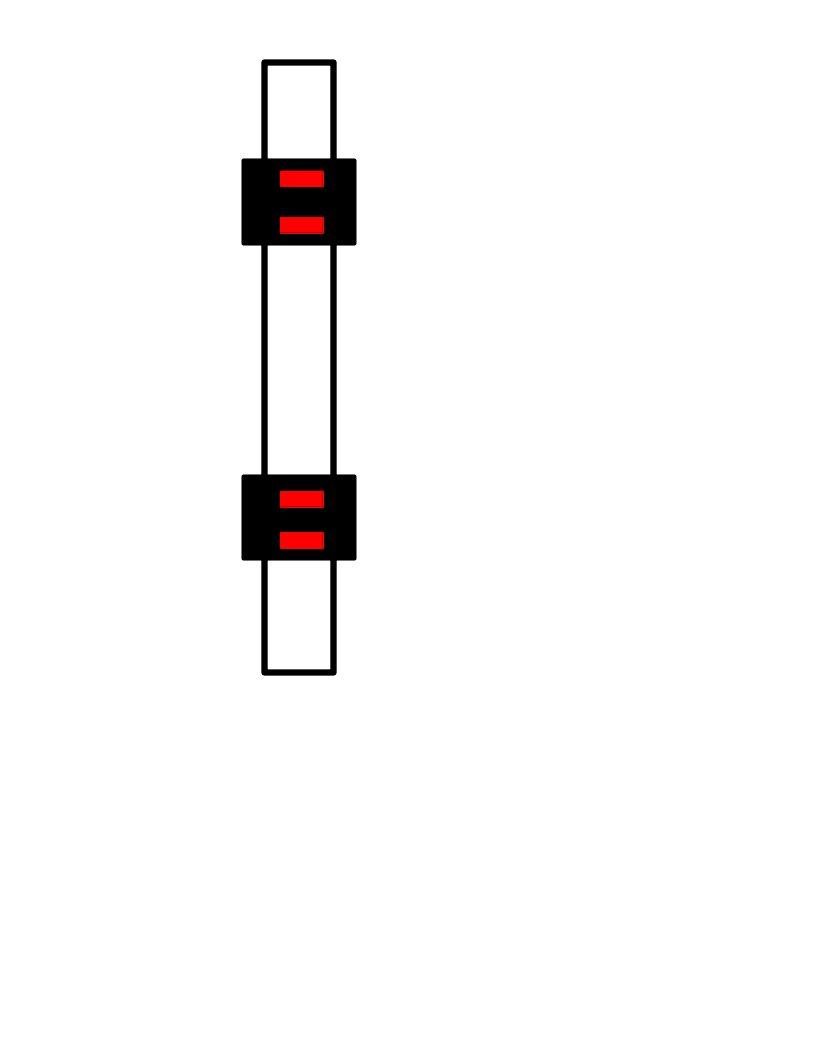
\includegraphics[width=0.23\textwidth,scale=0.2]{reticules.png}
\caption{\label{fig:reticules}Reticules}
\end{wrapfigure}

Reticule placement does not directly specify the level being controlled.  Level control is relative to the reticules and may be set to maintain a level at an offset above or below the level of the reticule. In the simplist case, however, it is convenient to position the reticule assembly so that the two red bars surround (above and below) the desired liquid level.  This corresponds to a zero offset for the liquid level to be maintained.

\subsubsection*{Vessels}

For each vessel, the
{\bf .previous}
file has a bounding box defining the region of the image where the meniscus will be visible, and intensity and contrast settings. Once
{\bf alevel.py}
reads this file, it will try to detect the horizontal liquid level in each of these regions using the contrast and intensity settings found in the file. However, if this fails it will vary each of these parameters by positive and negative factors in 10\% increments until it gets a good reading (or a specified number of attempts have been made).  With the {\bf update} option,
{\bf alevel.py}
will re-write the new values to the
{\bf .previous}
file.

\subsection*{Lighting}

The various EvoStat vessel holders shine light from bright green LEDs up into the liquid containers. When liquids are clear (e.g. uninoculated), this results in a reflection off the meniscus which can be used to determine the liquid level. However, the system works most reliably with the turbidity of a growing culture which is the primary mode of EvoStat operation.  Until the image processing has been improved, we should consider that accurate level readings will only occur when there is active culture in the vessels (e.g. not during setup and sterility testing).

Level readings also fail when the EvoStat chamber is opened, and therefore exposed to normal room lighting.  While the ability to darken the room can substitute for a closed chamber, we haven't had that luxury since being evicted from the Tod Vision's gardening tool shed in the Genome Sciences Building.

If a good level reading is not possible, calls to the level monitoring program return no results and the EvoStat reacts as if the last good reading was repeated.  As with all other parts of the EvoStat, the system is designed to operate with the current settings through any loss of telemetry.

\subsection*{Growth Conditions}
Under actual growth conditions, the liquids are turbid and create a lot of scattered light.  The LEDs below the vessel must be bright enough to completely illuminate the contents.  This is particularly important for the large, upper chamber because the light source is at the bottom of the 2-liter container. In particular, we do not see a high-contrast meniscus when the volume is near the overflow drain (1.5 liter level).

\section*{Next Steps}

Now that the level reporting program is relatively stable, a complete code-review re-write is in order.  Duplicated code can be eliminated in the horizontal line detection and image amplification subroutines. Red/reticule and Green/Level readings had minor differences which were best debugged using separate implementations.

Produce level information in resolution independent coordinates so that they are the same whether a 640x480 or 1280x1024 image is available. Or, alternately, provide image resolution information with the data and allow the recieving program to do the coordinate mapping.

\begin{enumerate}[itemsep=1pt, topsep=2pt, partopsep=0pt]
\item Review/re-write code: 800 lines of Python, can probably be halved.
\item Make level data resolution independent
\item Automate camera settings under Windows\textsuperscript{\textregistered}
\end{enumerate}

\bibliographystyle{unsrt}
\bibliography{alevel}{}

\pagebreak

\section{Appendix: alevel.py source code}
\newcommand*{\SrcPath}{../..}
\lstinputlisting[language=Python]{\SrcPath/alevel.py}
\end{document}











\input{\MyPath/chap1/ch1.tex}
